Graficando i dati ottenuti nel paragrafo precedente, ci si accorge immediatamente (si veda
la figura \ref{fig:lunghezza_periodo}) che il periodo del pendolo dipende dalla lunghezza
del suo filo, come correttamente previsto dalla teoria. Tuttavia la dipendenza non è lineare.

\begin{SCfigure}
    \centering
    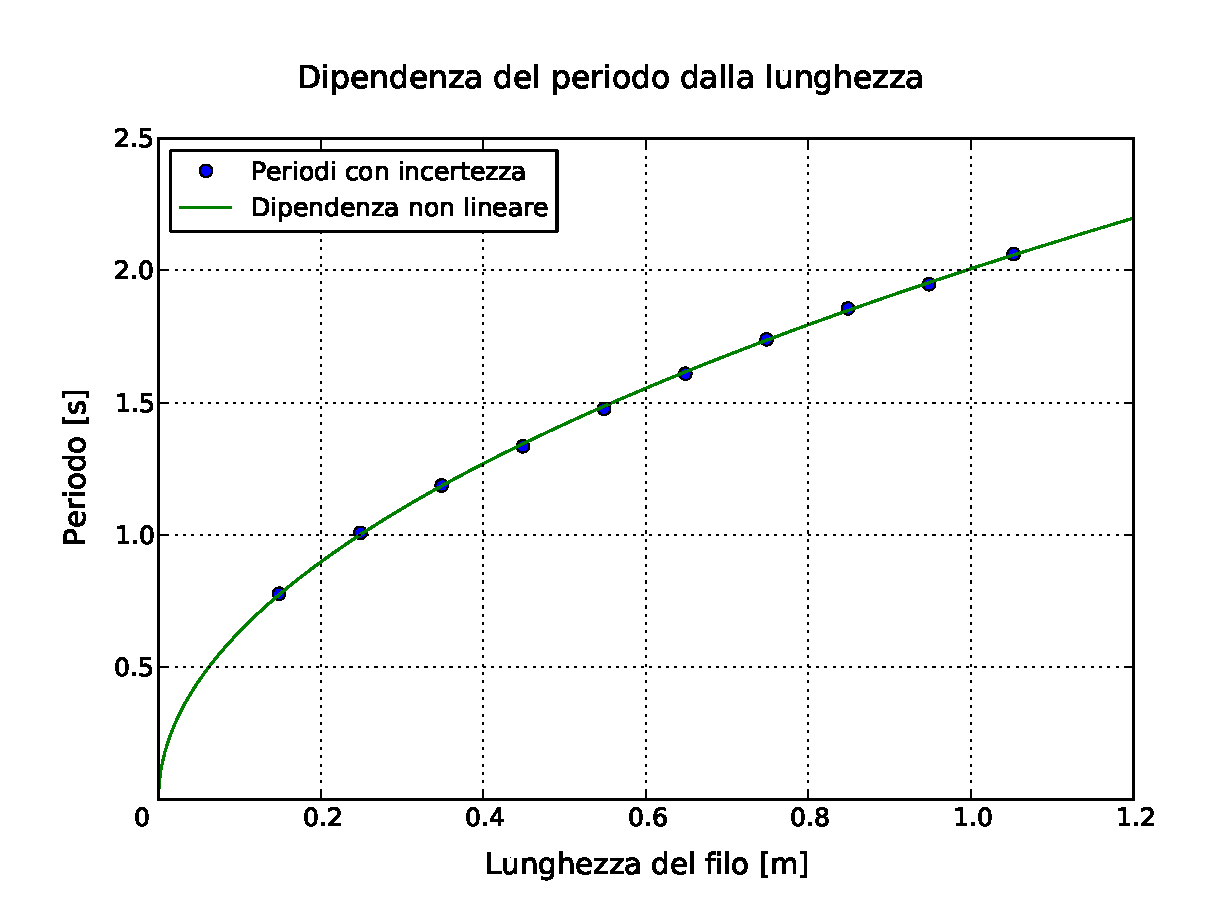
\includegraphics[width=120mm]{immagini/lunghezza_periodo.pdf}
    \caption{}
    \label{fig:lunghezza_periodo}
\end{SCfigure}

Osserviamo che i punti del grafico sembrano seguire una legge del tipo:

\begin{equation}
    \mathcal{T} = a\ell^b
\end{equation}
%
dove a e b sono due costanti.
